\providecommand{\main}{..}
\documentclass[\main/main.tex]{subfiles}

\begin{document}
\graphicspath{{img/}{ble_mesh/img/}}

\chapter{Bluetooth mesh}

\section{Mesh system architecture}

Bluetooth mesh networking provides the foundation to create a truly large-scale device network, allowing tens, hundreds or even thousands of wireless devices to communicate with each other reliably and securely.

Compared with other topologies, in a mesh network, each node may have a direct communication link with many nodes. This brings the robustness to the network against the single point of failure problem but also makes it harder to manage. Figure \ref{fig:Mesh topology} illustrates a basic example of mesh topology.

\begin{figure}[H]
    \begin{center}
        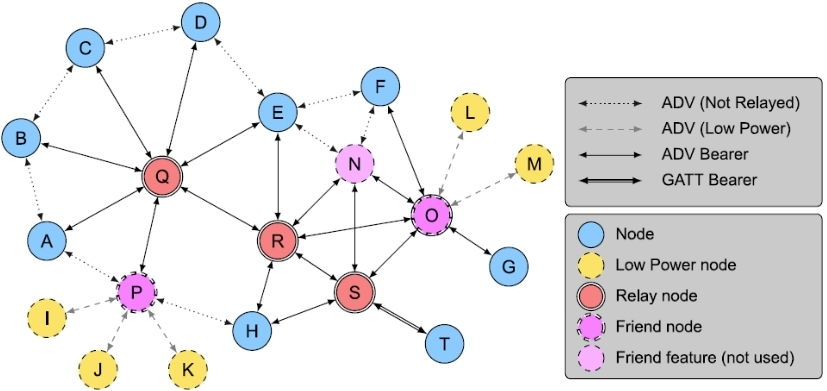
\includegraphics[scale=0.7]{mesh_topology.jpg}
    \end{center}
    \caption{Mesh topology}
    \label{fig:Mesh topology}
\end{figure}

This section provides an overview of the mesh network operation and layered system architecture.
\subsection{Layered architecture}
The Mesh Profile specification is defined as a layered architecture as shown in \ref{fig:ble_mesh_layered_architecture}.

\begin{figure}[H]
    \begin{center}
        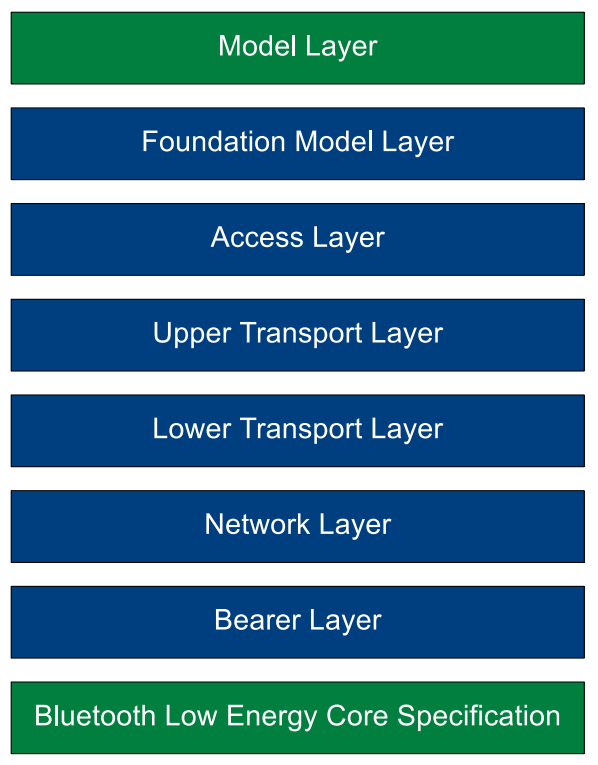
\includegraphics[scale=0.25]{ble_mesh_layered_architecture.png}
    \end{center}
    \caption{Mesh system architecture}
    \label{fig:ble_mesh_layered_architecture}
\end{figure}

\subsection{Model layer}
The Model layer defines models that are used to standardize the operation of typical user scenarios and are defined in the Bluetooth Mesh Model specification or other higher layer specifications. Examples of higher layer model specifications include models for lighting and sensors.
\subsection{Foundation Model layer}
The Foundation Model layer defines the states, messages, and models required to configure and manage a mesh network.
\subsection{Access layer}
The access layer defines how higher layer applications can use the upper transport layer. It defines the format of the application data; it defines and controls the application data encryption and decryption performed in the upper transport layer; and it checks whether the incoming application data has been received in the context of the right network and application keys before forwarding it to the higher layer

\subsection{Upper transport layer}
The upper transport layer encrypts, decrypts, and authenticates application data and is designed to provide confidentiality of access messages. It also defines how transport control messages are used to manage the upper transport layer between nodes, including when used by the Friend feature.

\subsection{Lower transport layer}
The lower transport layer defines how upper transport layer messages are segmented and reassembled into multiple Lower Transport PDUs to deliver large upper transport layer messages to other nodes. It also defines a single control message to manage segmentation and reassembly.

\subsection{Network layer}
he network layer defines how transport messages are addressed towards one or more elements. It
defines the network message format that allows Transport PDUs to be transported by the bearer layer.
The network layer decides whether to relay/forward messages, accept them for further processing, or
reject them. It also defines how a network message is encrypted and authenticated.

\subsection{Bearer layer}
The bearer layer defines how network messages are transported between nodes. There are two bearers
defined, the advertising bearer and the GATT bearer. Additional bearers may be defined in the future.

\section{Overview of mesh operation}

The mesh network operation defined by this specification is designed to:
\begin{itemize}
    \item enable messages to be sent from one element to one or more elements;
    \item allow messages to be relayed via other nodes to extend the range of communication;
    \item secure messages against known security attacks, including eavesdropping attacks, man-in-themiddle attacks, replay attacks, trash-can attacks, brute-force key attacks, and possible additional security attacks not documented here;
    \item work on existing devices in the market today;
    \item deliver messages in a timely manner;
    \item continue to work when one or more devices are moved or stop operating;
    \item have built-in forward compatibility to support future versions of the Mesh Profile specification
\end{itemize}

This specification defines a managed-flood-based mesh network, which uses broadcast channels to
transmit messages so that other nodes can receive messages and relay these messages; thus extending
the range of the original message. Any device in a managed-flood mesh network can send a message at
any time as long as there is a sufficient density of devices that are listening and relaying messages.
Enhancements to add routing functionality and define a routing-based mesh network may be considered
for a future revision of this specification.
There are a number of methods used by this specification to restrict the unlimited relaying of messages in
a managed-flood mesh network. The two main methods used are the network message cache method
and the time to live method.
The network message cache is designed to prevent devices from relaying previously received messages
by adding all messages to a cached list. When a message is received, it is checked against the list and
ignored if already present. If not already received, then it is added to the cache so that it can be ignored in
the future. To prevent this list from becoming too long, the number of messages that are cached is limited
by implementation.
Each message includes a Time to Live (TTL) value that limits the number of times a message can be
relayed. Each time a message is received and then relayed (up to a maximum of 126 times) by a device,
the TTL value is decremented by 1.

\section{Node software architecture}

A BLE mesh capable device which is not a member of any BLE mesh network is called \textbf{unprovisioned device}. After joining a  network, it is eligible to call it a \textbf{node}. The action of making an unprovisioned device become a node is called \textbf{provision}.

There may be more than one kind of node existing in a BLE mesh network. Each kind plays a different role working together to make the network run. Five types of nodes are defined in the \textbf{Mesh Networking Specifications} published by Bluetooth SIG (Bluetooth Special Interest Group).
\begin{itemize}
    \item Normal node (usually called node)
    \item Relay node
    \item Low power node
    \item Friend node
    \item Proxy node
\end{itemize}

Figure \ref{fig:Node software architecture} shows the software architecture of a node. In application implementation, understanding each component is required because there are the needs of defining each of them in memory. The details of each component is discussed in the following subsection.
\begin{figure}[H]
    \begin{center}
        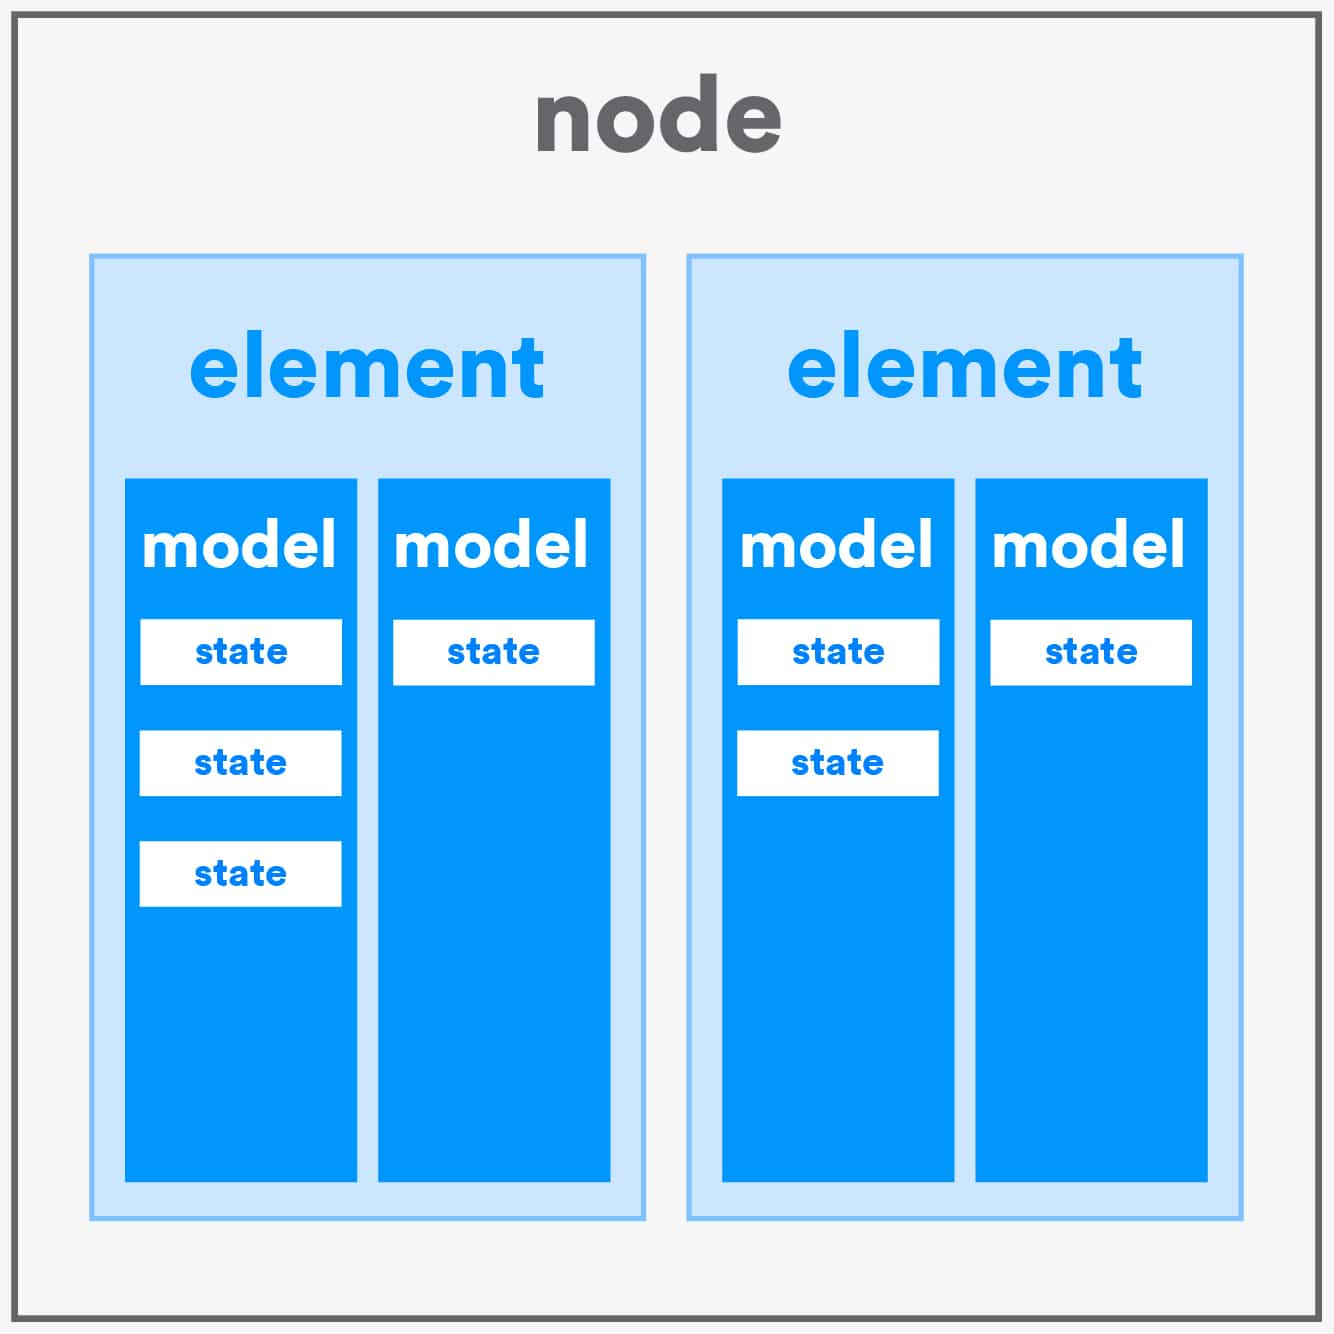
\includegraphics[scale=0.15]{node_software_architecture.jpg}
    \end{center}
    \caption{Node software architecture}
    \label{fig:Node software architecture}
\end{figure}

\subsection{Element}
In a BLE mesh network, a node is a physical device consisting of one or more elements. Compared to the node, an element is the logic component of the network. By this way, a mesh network is logically a group of elements communicating with others. Because an element is a network entity, it will be addressed uniquely in the mesh network.

Why element is defined? Let's think of a device with more than one light bulb, by introducing the element concept, each light bulb may be considered as an element of the network. This makes the network more flexible and removes application layer special muxing.

\subsection{Model}
The communication channel between elements is the model. A model can subscribe to a topic or publish data to a topic that may be subscribed by other models. The publish/subscribe pattern brings the ability to  communicate with multiple devices with a single message without knowing the exact address of such devices. Figure \ref{fig:BLE mesh publish/subscribe model} illustrates the publish/subscribe pattern. 

\begin{figure}[H]
    \begin{center}
        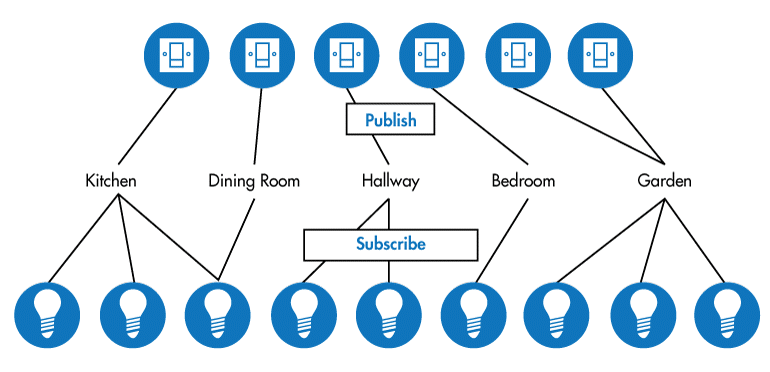
\includegraphics[scale=0.4]{ble_mesh_pub_sub.png}
    \end{center}
    \caption{BLE mesh publish/subscribe model}
    \label{fig:BLE mesh publish/subscribe model}
\end{figure}

\subsection{State}
A state is an internal variable inside the model. In the simple case, it may save a state of the element such as the on/off state of a light bulb.

\section{Security \cite{web_bluetooth_mesh_security_overview}}
One of the most discussed issues related to the Internet of Things (IoT) is security. From agriculture to hospitals, from residential smart homes to commercial smart buildings, and from power stations to traffic management systems, IoT systems and technologies will touch many parts of the world we live in. Security breaches in IoT systems could have catastrophic consequences.

Bluetooth mesh networking was designed with security as its number one priority and from the ground up. In this article, you’ll get an overview of the key security features and the security issues addressed. Further articles in the series will examine aspects of Bluetooth mesh networking security in more detail

\subsection{Security in Bluetooth Mesh Networking is mandatory}
Bluetooth Low Energy (LE) GATT devices may implement a range of security measures as defined in the Bluetooth core specification. It’s the responsibility of the product designer to decide what security measures are required and it’s permissible to decide to adopt none of the available security features at all. In other words, security in Bluetooth Low Energy GATT is optional. This makes sense if we’re talking about the security of a single device and its connection with one other device, provided the product designer performs their risk assessment correctly. However, security in Bluetooth mesh networking is concerned with the security of more than individual devices or connections between peer devices; it’s concerned with the security of an entire network of devices and of various groupings of devices in the network.

Consequently, security in Bluetooth mesh networking is mandatory.

\subsection{Bluetooth Mesh Networking Security Fundamentals}
The following fundamental security statements apply to all Bluetooth mesh networks.

\begin{table}[H]
    \centering
    \begin{tabular}{|m{0.3\textwidth}|m{0.65\textwidth}|}
    \hline
    % \centering  &  \centering  \\\hline
    \multicolumn{1}{|>{\centering\arraybackslash}m{0.3\textwidth}|}{\textbf{Security statements}} & \multicolumn{1}{>{\centering\arraybackslash}m{0.65\textwidth}|}{\textbf{Description}}\\
    \hline

    Encryption and Authentication &  All Bluetooth mesh messages are encrypted and authenticated. \\ \hline
    Separation of Concerns & Network security, application security, and device security are addressed independently.\\ \hline
    Area Isolation & A Bluetooth mesh network can be divided into subnets, each cryptographically distinct and secure from the others. \\ \hline
    Key Refresh & Security keys can be changed during the life of the Bluetooth mesh network via a Key Refresh procedure. \\ \hline
    Message Obfuscation & Message obfuscation makes it difficult to track messages sent within the network and, as such, provides a privacy mechanism to make it difficult to track nodes. \\\hline
    Replay Attack Protection & Bluetooth mesh security protects the network against replay attacks. \\\hline
    Trashcan Attack Protection & Nodes can be removed from the network securely, in a way which prevents trashcan attacks. \\\hline
    Secure Device Provisioning & The process by which devices are added to the Bluetooth mesh network to become nodes is a secure process. \\\hline
    \end{tabular}
    \caption{Security statements}
    \label{table:security_statements}
\end{table}

\subsection{Separation of Concerns and Security Keys}
At the heart of Bluetooth® mesh security are three types of security keys. These keys provide security to different aspects of the Bluetooth mesh network and achieve a critical capability in Bluetooth mesh networking security called a separation of concerns.

Consider a mesh light which acts as a relay. In its capacity as a relay, it may find itself handling messages relating to the building’s Bluetooth mesh door and window security system. A light has no business accessing and processing the details of these messages, but it does need to relay them to other nodes.

To deal with this potential conflict of interest, Bluetooth mesh uses different security keys called \textbf{AppKeys} for securing messages at the network layer from those used to secure data relating to specific applications, such as lighting, physical security, heating, etc.

All nodes in a Bluetooth mesh network possess one or more \textbf{Network Keys (NetKey)}, each corresponding to a subnet which may be the primary subnet. It’s possession of a network key which makes a node a member of the network. Network Encryption Keys and Privacy Keys are derived directly from the NetKey.

Being in possession of a NetKey allows a node to decrypt and authenticate up to the Network Layer so that network functions, such as relaying, can be carried out. It does not allow application data to be decrypted.

Each node also has a unique security key called the \textbf{Device Key or DevKey}. The DevKey is used in the provisioning and configuration of the node.

\subsection{Area Isolation}
Possession of the primary NetKey defines membership of and grants access to the Bluetooth® mesh network. But it’s also possible to divide the network into distinct subnets, each with its own subnet key. This means that only devices in possession of a given subnet key can communicate with other devices that are members of that subnet. Subnet keys can be created and assigned on an adhoc basis too. A great example is isolating nodes in different hotel rooms from each other.

\subsection{Node Removal, Key Refresh, and Trashcan Attacks}
As described above, nodes contain various Bluetooth® mesh security keys. Should a node become faulty and need to be disposed of, or if the owner decides to sell the node to another owner, it’s important that the device and the keys it contains cannot be used to mount an attack on the network the node was taken from.

A procedure for removing a node from a network is defined. The Provisioner application is used to add the node to a reject list and then a Key Refresh Procedure is initiated.

The Key Refresh Procedure issues all nodes in the network, except those which are members of the reject list, new network keys, application keys, and all related, derived data. In other words, the entire set of security keys which form the basis for network and application security are replaced.

As such, a node which was removed from the network, and which contains an old NetKey and old set of AppKeys, is no longer a member of the network and poses no threat.

\subsection{Privacy}
A Privacy Key, derived from the NetKey, is used to obfuscate network PDU header values, such as the source address. Obfuscation ensures that casual, passive eavesdropping cannot be used to track nodes and the people using them. It also makes attacks based upon traffic analysis difficult.

\subsection{Replay Attacks}
In network security, a replay attack is a technique whereby an eavesdropper intercepts and captures one or more messages and simply retransmits them later, with the goal of tricking the recipient into carrying out something which the attacking device is not authorized to do. A commonly cited example is a car’s keyless entry system being compromised by an attacker who intercepts the authentication sequence between the car’s owner and the car, later replaying those messages to gain entry to the car and steal it.

Bluetooth mesh networking protects against replay attacks by using two network PDU fields called the Sequence Number (SEQ) and IV Index. Elements increment the SEQ value every time they publish a message. A node which receives a message from an element containing an SEQ value less than or equal to that of the last valid message will discard it since it likely relates to a replay attack. Similarly, IV Index is a separate field considered alongside SEQ. IV Index values within messages from a given element must always be equal to or greater than the last valid message from that element.

\section{Mynewt nimble}
Apache NimBLE is an open-source Bluetooth 5.1 stack (both Host and Controller) that completely replaces the proprietary SoftDevice on Nordic chipsets. It is part of Apache Mynewt project.

Features highlight:
\begin{itemize}
    \item Support for 251 byte packet size
    \item Support for all 4 roles concurrently - Broadcaster, Observer, Peripheral and Central
    \item Support for up to 32 simultaneous connections.
    \item Legacy and SC (secure connections) SMP support (pairing and bonding).
    \item Advertising Extensions
    \item Coded (aka Long Range) and 2M PHYs.
    \item Bluetooth Mesh.
\end{itemize}

\subsection{Bearers}
Mesh Profile specification allows two kinds of bearers for transmitting data:

\begin{itemize}
    \item Advertising Bearer: \begin{itemize}
        \item Uses LE advertising to broadcast messages to all nodes that are listening at this time
        \item Uses non-connectable advertising only
        \item 29 octets of network message
    \end{itemize}
    \item GATT Bearer: \begin{itemize}
        \item Uses LE Connections to send messages
        \item Uses standard GATT service (one for Provisioning and one for Proxy)
    \end{itemize}
\end{itemize}

\subsection{Provisioning}
Provisioning is a process of adding an unprovisioned device to a mesh network managed by a Provisioner. A Provisioner provides the unprovisioned device with provisioning data that allows it to become a mesh node (network key, current IV index and unicast address). A Provisioner is typically a smart phone or other mobile computing device.

\subsection{Models}
Models define basic functionality of nodes on a mesh network. Mesh Profile Specification defines foundation models used to configure and manage network. Mesh Model Specification includes models defininig functionality that is standard across device types. Those consists of:
\begin{itemize}
    \item Generics - root models \begin{itemize}
        \item On/Off
        \item Level
        \item Battery Server
        \item Location
        \item Client Property
        \item and others
    \end{itemize}
    \item Sensors - defines a standard way of interfacing with sensors
    \item Time and Scenes - defines a set of functionalities related to time and saved states on devices
    \item Lighting - defines a set functionalities related to lighting control
\end{itemize}
Complex models e.g. Lighting may contain other models eg Generic On/Off. Figure \ref{fig:ble_mesh_lightning_model} shows an example of Light Lightness Server Model.

\begin{figure}[H]
    \begin{center}
        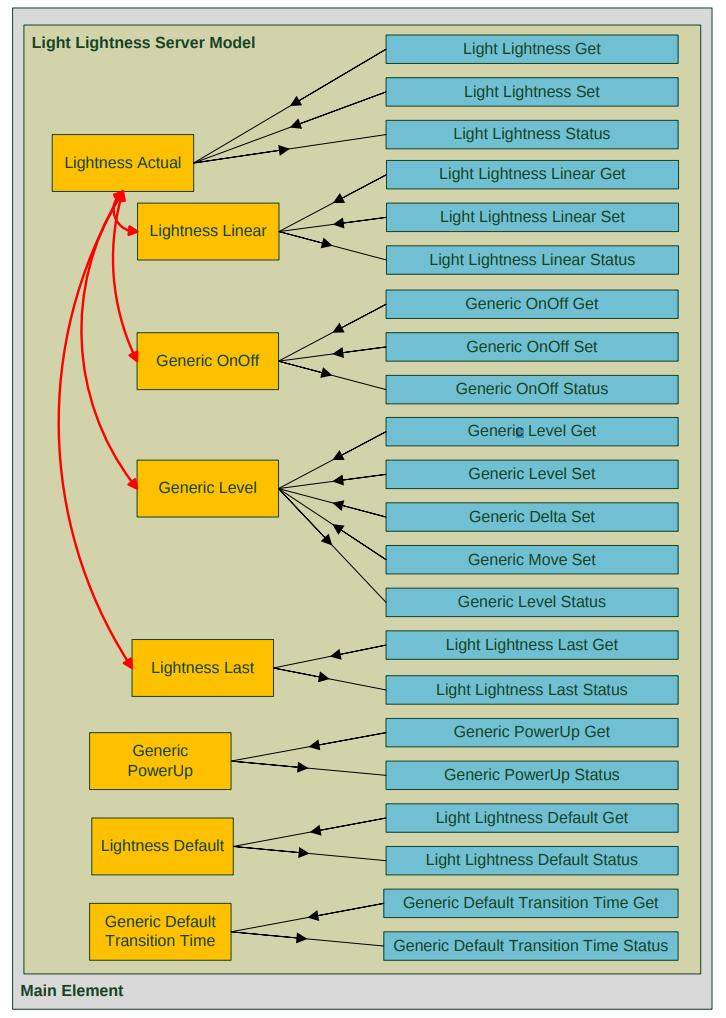
\includegraphics[scale=0.3]{ble_mesh_lightning_model.jpg}
    \end{center}
    \caption{BLE mesh lightning model}
    \label{fig:ble_mesh_lightning_model}
\end{figure}

\section{Using Bluetooth mesh for best-effort broadcast service}

\begin{figure}[H]
    \begin{center}
        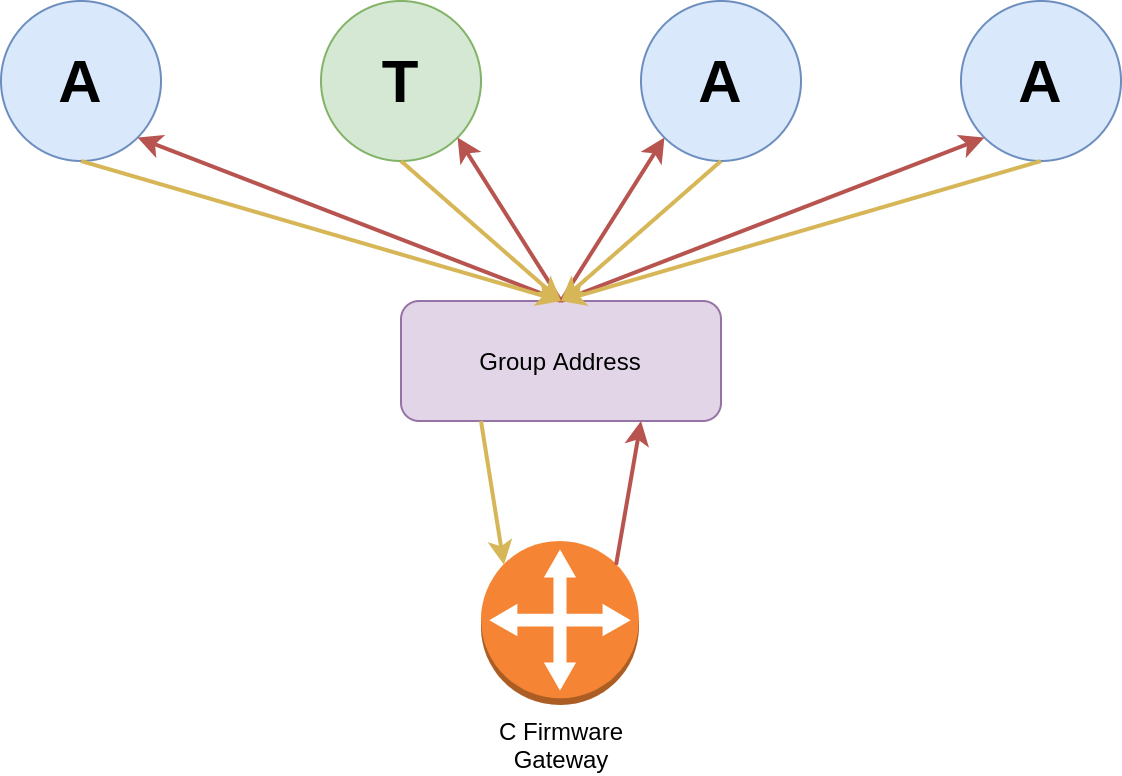
\includegraphics[scale=0.3]{ble_mesh_comunication.png}
    \end{center}
    \caption{ble mesh communication}
    \label{fig:ble_mesh_comunication}
\end{figure}

\section{Custom nRF Mesh Android application}
\bib
\end{document}